\chapter{Specifikace a návrh platformy pro VNF}

V předešlé kapitole byla vysvětlena základní problematika, která souvisí s virtualizací síťových funkcí, cloud computingem a softwarově definovanými sítěmi. Zároveň byla popsána referenční architektura frameworku pro virtualizaci síťových funkcí. Tato kapitola bude již věnována konkrétnímu příkladu využití virtuálních síťových funkcí v cloudovém prostředí. Nejprve zde popsána navržená architektura pro privátní cloudovou platformu využívající virtualizaci síťových funkcí, kterou mohou využívat všichni její uživatelé. Pro tuto cloudovou platformu a pro její uživatele byli navrženy dva příklady virtuálních síťových funkcí. U obou příkladů jsou uvedeny scénáře a způsob jakým jsou navrženy.

\section{Požadavky na framework}

//Opensource

\section{Požadavky na životní cyclu VNF}

//automatic creating of VNF + with all infrastructure

//automatic konfiguration + 

//automatic rekonfiguration

\section{Použité technologie}

\subsection{OpenStack}

//Todo Proč jsem si vybral OpenStack??

OpenStack je open-source platformou umožňující postavit IaaS cloud, který může být nainstalován i na běžném hardwaru. Toto řešení má za cíl vytvořit dostupnou cloudovou platformu, která bude splňovat všechny potřeby privátních a veřejných cloudů nezávisle na velikosti řešení. \cite{OpenStack}

Celá stavba systému OpenStack se skládá z několika na sobě nezávislých projektů (modulů), které řeší různé oblasti cloudové platformy. Tyto projekty mezi sebou komunikují pomocí otevřených API a mohou být spravovány pomocí dashboardu. Celé administrace OpenStacku může být prováděna přes webově rozhraní, příkazovou řádku či přímo pomocí příkazů zaslaných do API. Celé toto řešení se vyznačuje jednoduchostí implementace, škálovatelností a rychlým vývojem nových vylepšení. Hlavními moduly OpenStacku jsou \cite{OpenStack} \cite{OpenStack2}:

\begin{itemize}
\item Keystone - identifikační služba používaná OpenStackem pro autorizaci a autentizaci. Ověřování probíhá pomocí tokenů. Uživatel přihlášením odesílá žádost na Keystone, který tento modul zpracuje, zjistí pověření a vytvoří token. Vytvořený token je poté odesílán s žádostí do ostatních služeb. Zde dojde ke komparaci tokenu se současnou přístupovou politikou a dojde ke zjištění, zdali má uživatel dostatečná oprávnění pro provedení požadovaného úkonu.
\item Glance - služba umožňující práci s virtuálními diskovými obrazy (imagy). Tyto obrazy mohou být uloženy na mnoha různých místech od lokálních systémových disků až po distribuované souborové systémy, jako je OpenStack Storage.
\item Nova - tento modul poskytuje výpočetní služby. Umožňuje tedy běh několika instancí virtuálních strojů na několika hostitelských strojích, nan kterých je nainstalována služba OpenStack compute. OpenStack podporuje hypervizory KVM, QEMU, VMware ESX, Hyper-V, Xen. 
\item Neutron - je služba pro správu všech síťových aspektů OpenStacku. Jedná se tedy o SDN komponentu. Neutron podporuje možnost rozšíření o tzv. pluginy, které umožňují využívat řešení třetích stran pro síťování.
\item Cinder - poskytuje infrastrukturu pro mapování volumů v OpenStacku.
\item Ceilometer - služba, která sbírá měřená data a monitoruje tak využívané zdroje.
\item Heat - umožňuje automatizovanou orchestraci virtuálních strojů na základě vytvořených templatů.
\item Horizon - představuje dashboard, který umožňuje cloudovým administrátorům a uživatelům spravovat různé zdroje a služby OpenStacku. Dashboard umožňuje interakci s OpenStackovým kontrolerem prostředníctvím API. 
\end{itemize}

\subsubsection{Heat}

\subsection{OpenContrail} 

OpenContrail je systém, který může být použit v mnoha síťových scénářích jako například v cloud networkingu nebo v sítích poskytovatele síťových služeb. V privátním cloudu, ve Virtual Private Cloud (VPC) a v IaaS se vyskytuje prostředí s velkým množstvím tenantů, kde několik tenantů sdílí stejné fyzické zdroje (server, uložiště, fyzickou síť). Každý tenant má přiřazeny vlastní logické zdroje (virtuální stroje, virtuální uložiště, virtuální sítě). Tyto logické zdroje různých tenantů musí být od sebe odděleny. Virtuální sítě v datacentrech mohou být také spojeny s fyzickou IP VPN nebo L2 VPN. \cite{OpenContrail}

OpenContrail je složen ze dvou hlavních komponent. První z nich je Controller, který je logicky centralizovaný, ale fyzicky distribuovaný. To znamená, že je složen z několika typů rolí a každý z nich má několik instancí z důvodu vysoké dostupnosti a horizontální škálovatelnosti. Tyto role mohou být fyzické servery nebo virtuální stroje. Tyto role jsou \cite{OpenContrail2}: 

\begin{itemize}
\item Configuration role - poskytuje north-bound REST API. Toto API může být použito pro konfiguraci systému nebo pro extrahování operačního stavu systému.
\item Control role - implementuje logicky centralizovanou část control planu.
\item Analytics role - je zodpovědný za sběr, porovnání a prezentaci analytických informací.
\end{itemize}

Další komponentou je vRouter, který má na starost přenos dat. VRouter běží na virtualizovaném serveru, na kterém běží hypervizor. Rozšiřuje fyzickou síť v datovém centru o virtuální overlay síť hostovanou ve virtualizovaných serverech. VRouter narozdíl od vSwitchů poskytuje směrování a služby vyšších vrstev. Data plane, tedy vRoutery mezi sebou, může používat různé technologie overlay jako MPLS over GRE, MPLS over UDP a VXLAN. Control plane protocol mezi Controllerem a fyzickým gateway routerem (nebo switchem) je BGP. Protokol používaný mezi Controllerem a vRoutery se nazývá XMPP. Obrázek č. \ref{fig:contrail} ukazuje schéma OpenContrailu.

\begin{figure}[h]
\begin{centering}
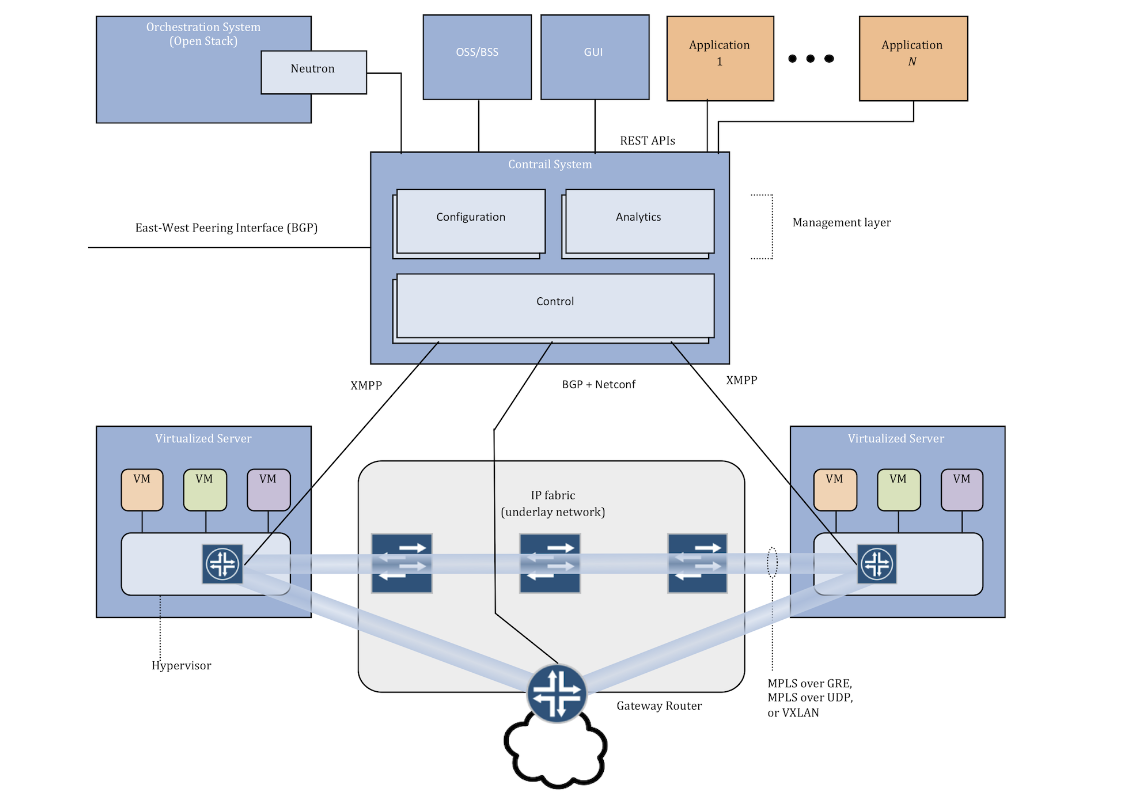
\includegraphics[scale=0.35]{images/contrail}
\par\end{centering}
\caption{Schéma OpenContrail, převzato z \cite{OpenContrail}\label{fig:contrail}}
\end{figure}

//Servisní instance v Opencontrailu

\subsection{SaltStack}

\subsection{Použitý software pro VNF}

//TODO co jsem si vybral za VNFka

Pokud se podíváme na trh s VNF u některých vendorů, tak zjistíme, že mnozí poskytují virtuální instance, které se dají použít pro účely VNF v této práci. Tato práce je zaměřena především na funkce firewallu a proto zde jsou uvedeny příklady pouze pro ně. Uvedeny jsou hlavně produkty největších a nejpoužívanějších poskytovatelů síťových prvků a také open-source firewall.

\begin{itemize}
\item Juniper vSRX - Jde o firewall od společnosti Juniper, který je obdobou jejich fyzického zařízení Juniper SRX. Jde virtuální instanci poskytující funkce pro firewall, routing a pokročilé bezpečností funkce pro poskytovale telekomunikačních služeb a větší společnosti. Toto VM je určené pro privátní, public i hybrid cloud. 
\item Fortigate-VM - Fortigate Virtual Appliances je řešení pro cloudové prostředí od společnosti Fortinet. Nabízí stejně funkce pro firewall jako jsou obsaženy ve Fortigate fyzických zařízeních.
\item Cisco ASAv - Společnost Cisco nabízí Adaptive Security Virtual Appliance (ASAv), která obsahuje stejný software jako fyzické ASA zařízení a vetšinu funkcí pro firewall, routing a VPN. 
\item PFSense - PFSense je open-source projekt, který má za cíl poskytnout firewall postavený na operačním systému FreeBSD, který může běžet na klasické architektuře jednodeskových počítaču. Toto řešení poskytuje všechny důležité vlastnosti komerčních firewallů, má jednoduché ovládání a je to otevřené řešení.
\end{itemize} 

Navrhnutá řešení v této práci předvádějí virtuální víťové funkce pro firewall a load balancing. Jsou zde ukázány celkem 3 scénáře případu užíti. Dva jsou zaměřeny na FwaaS (Firewall as a Service) a jeden na LbaaS (Load balancer as a Service). Všechna řešení jsou vytvořena pomocí Heat templatů, které se spouští v prostředí OpenStack.

Aby mohla být nějaká VNF vůbec vytvořena, tak musel být nejprve zvolen software či operační systěm, který má požadovanou funkci implementovánu. Pro tyto účely byly použity následující řešení:

\begin{itemize}
\item PFSense – open-souce firewall založený na operačním systému FreeBSD.
\item FortiGate-VM – je plnohodnotně vybavený Fortigate firewall zabalený jako virtualní instance.
\item Neutron Agent-HAproxy – je velmi rychlé a spolehlivé řešení nabízející vysokou dostupnost, load balancing a proxy pro aplikace založené na TCP a HTTP
\end{itemize}

Následující diagram znázorňuje logickou architekturu navrženého řešení dle referenční architektury zmíněné v kapitole 2.4. OpenStack spolu s OpenContrailem poskytují NFV infrastrukturu jednotlivé VNF jsou řízeny pomocí Heat.

\section{Architektura použitého frameworku}

Architektura navrženého řešení byla implementována pomocí cloudové platformy OpenStack a SDN řešení OpenContrail. Obrázku č. \ref{fig:VNF_overview} znázorňuje tyto technologie v souvislosti s referenční architekturou popsanou v kapitole \ref{sub:architektura}. Je nutné říci, že obě technologie nezapadají přímo do jedné z částí referenční architektury. Naopak v některých případech se překrývají nebo se v ní doplňují.

\begin{figure}[h]
\begin{centering}
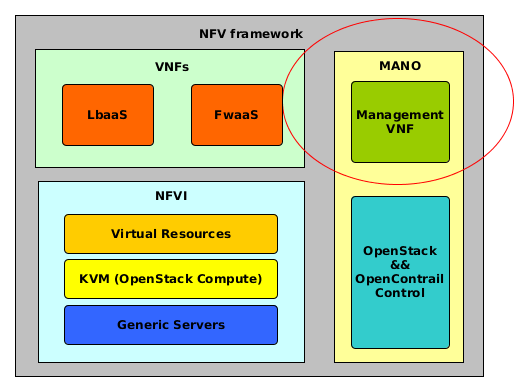
\includegraphics[scale=0.51]{images/VNF_overview}
\par\end{centering}
\caption{Architektura NFV řešení\label{fig:VNF_overview}}
\end{figure}

OpenStack byl zvolen, protože se jedná o největší open-source cloudovou platformu na světě. OpenStack tvoří část správy infrastruktury. Hardwarová vrstva infrastruktury se může skládat z libovolných serverů, na kterých je nainstalován KVM hypervizor. Tento hypervizor tvoří virtuální vrsvu a byl vybrán, protože je nejčastěji používán společně s OpenStackem. Avšak v případě potřeby by zde mohl být použit i jiný hypervizor, pokud bude zachována kompatibilita vůči OpenStacku.

OpenStack spravuje převážně zdroje týkající se výpočeního výkonu (Compute) a uložiště (Storage). Tyto zdroje následně přiděluje dle potřeby virtuálním instancím nebo v našem případě instancím, které slouží jako VNF. Bylo však nutné zvolit řešení, které se bude starat o síťování.

Speciálně pro vyřešení síťování v této infrastruktuře je součástí řešení OpenContrail. Díky tomu je možné vytvářet overlay sítě pomocí VXLAN či MPLS over GRE, kterými jsou dynamicky propojovány jednotlivé VM a VNF. 

Jednotlivá VNF mohou být v OpenContrailu vytvořena pomocí tzv. Servisních Instance a Servisní Templatů. Ty budou v této práci použity pro vytvoření VNF sloužící jako firewally a budou podrobně popsány v kapitole věnující se vytváření této služby.

Další součástí, která musela být v architektuře navrhnuta, je způsob řízení a správy jednotlivých VNF. Zde se muselo jednat o řešení, jakým automaticky vytvořit a popřípadě i smazat všechny potřebné části potřebné pro VNF. Pro tuto část byl zvolen Heat. Heat je část OpenStacku, která slouží pro automatickou orchestraci. Ten bude v tomto návrhu zastávat roli VFN managera, pomocí kterého budou jednotlivé VNF spravovány. Avšak dalo by se říci, že do této role spadá i OpenContrail, protože právě on umožnuje také spravovat jednostlivá VNF za běhu.  

Heat je hlavní projekt v OpenStacku pro orchestraci. Umožňuje uživatelům popsat nasazení komplexních cloudových aplikací v jednom textovém souboru, který se nazývá Heat template. Tyto soubory se dají předat heat enginu, který podle nich dokáže automaticky vytvořit požadované zdroje v OpenStacku i v OpenContrailu. 

\begin{figure}[h]
\begin{centering}
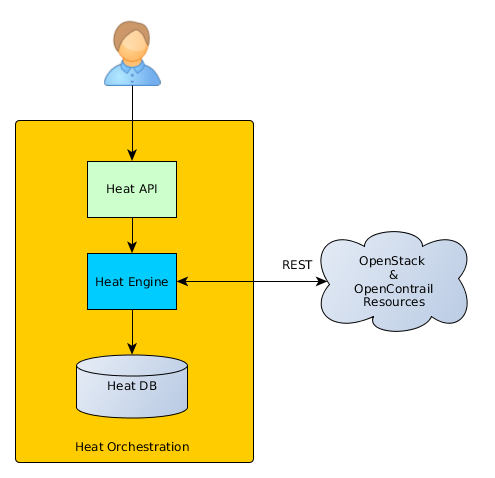
\includegraphics[scale=0.41]{images/heat_engine}
\par\end{centering}
\caption{Popis heat orchestrace\label{fig:heat_engine}}
\end{figure}

Z toho návrhu je patrné, že zde není implementovaný NFV orchestrator. Je to z důvodu toho, že pro účely řešení virtuálních síťových funkcí na cloudové platformě OpenStack s OpenContrailem, která je navržena v této práci, není tato část potřeba.

\subsection{Fyzicka topologie - underlay}\label{sub:interaction}

Celá testovací topologie se skládala z 4 serverů. Jeden server

\begin{figure}[h]
\begin{centering}
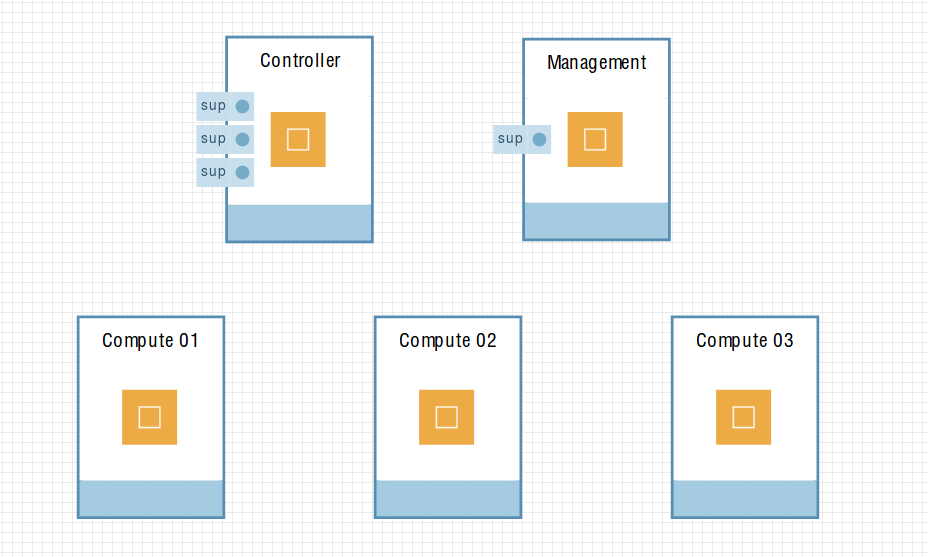
\includegraphics[scale=0.41]{images/ravello_topologie}
\par\end{centering}
\caption{Testovací topologie\label{fig:ravello_topologie}}
\end{figure}

